
\begin{TP}[Les vacances de Polo]

Ci-dessous un repère quadrille la carte de France.

\begin{center} 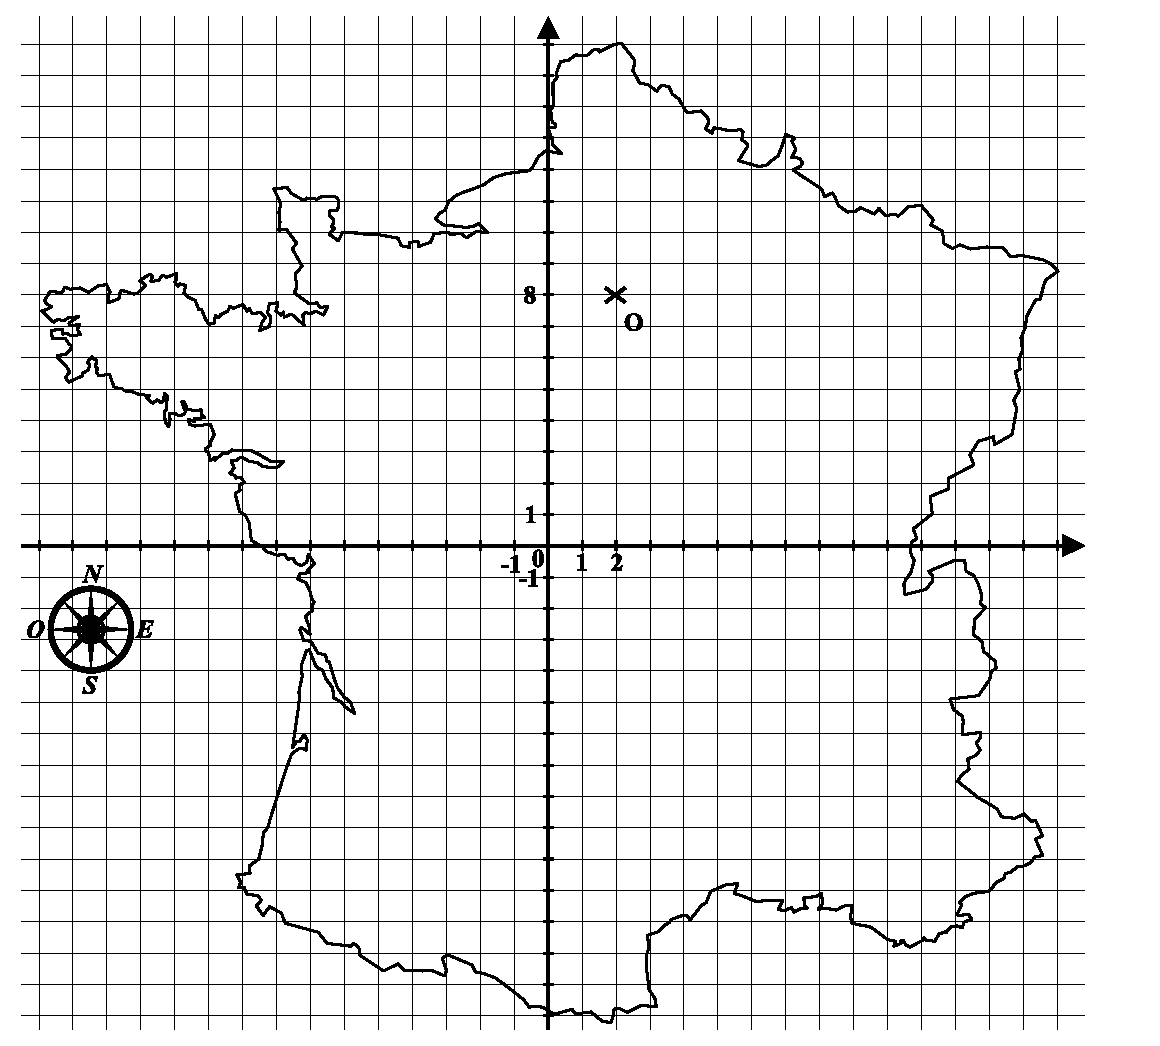
\includegraphics[width=12cm]{carteNOES} \end{center}

\begin{enumerate}
 \item Déterminez les coordonnées des points $A$, $B$, $C$, $D$, $E$, $F$, $G$, $H$, $I$, $J$, $K$, $L$, $M$, $N$, $O$, $P$, $R$, $S$ et $T$ sachant que :
 \begin{itemize}
  \item $A$ a pour abscisse $5$ et pour ordonnée $10$ ;
  \item $B$ a pour abscisse $-3$ et pour ordonnée $11$ ;
  \item L'ordonnée de $C$ est $-11$ et son abscisse est $5$ ;
  \item $D(-7 ; -1)$ et $E(3,5 ; 0)$ ;
  \item $F$ a pour ordonnée $-10$ et est aussi à l'Ouest que possible ;
  \item $G(-14 ; 7,5)$ ;
  \item $H$ a la même abscisse que $D$ et la même ordonnée que $G$ ;
  \item $I$ ne peut pas être plus au Nord ;
  \item La droite $(IB)$ (droite passant par les points $I$ et $B$) coupe l'axe des ordonnées au point $J$ ;
  \item Le point $K$ est le symétrique de $J$ par rapport à l'axe des abscisses ;
  \item $L$ est au bord de la mer et a la même ordonnée que $K$ ;
  \item $M$ a pour ordonnée $7$, et est aussi à l'Est que possible ;
  \item L'abscisse de $N$ est égale à l'ordonnée de $A$, et son ordonnée est l'opposée de l'abscisse de $C$ ;
  \item $O$ se lit sur la carte ;
  \item $P$ est à l'intersection des droites $(MN)$ et $(LC)$ ;
  \item $R$ est sur la droite $(KG)$, et son abscisse est égale à son ordonnée ;
  \item $S$ a pour abscisse $7$ et est sur la droite $(PR)$ ;
  \item $T$ et $S$ ont la même ordonnée, mais l'abscisse de $T$ est l'opposée de l'abscisse de $S$.
  \end{itemize}
 \item Chaque point sur la carte correspond à une des villes suivantes :
  \begin{colitemize}{3}
   \item Paris ;
   \item Etretat ;
   \item Moulins ;
   \item Lyon ;
   \item Annecy ;
   \item Montpellier ;
   \item Bordeaux ;
   \item Le Mont Saint-Michel ;
   \item La Rochelle ;
   \item Grenoble ;
   \item Perpignan ;
   \item Royan ;
   \item Brest ;
   \item Le Touquet ;
   \item Dunkerque ;
   \item Tarascon-sur-Ariège ;
   \item Reims ;
   \item Strasbourg ;
   \item Biarritz.
     \end{colitemize}
   À l’aide de votre atlas et de la liste ci-dessus, retrouvez et écrivez pour chaque point la ville qui lui correspond.
 \item Sachant que Polo se rend au point $T$, où ira-t-il en vacances cette année?
 \item Parmi les villes que vous venez de placer, la distance entre la ville la plus au Nord de la carte et celle la plus au Sud située en bord de mer correspond environ à 1000 km.
 
Sachant que Polo part de Reims, calculez approximativement la distance (en kilomètres et en ligne droite) qui sépare Polo de son lieu de vacances ?
  \end{enumerate}
\end{TP}

%%%%%%%%%%%%%%%%%%%%%%%%%%%%%%%%%%%%%%%%%%%%%%%%%%%%%%%%%%%%%%%%%%%

\begin{TP}[Bataille navale]

\begin{enumerate}
 \item Chaque groupe trace un repère d'unité 1 cm pour chaque axe. Les graduations pour l'axe des abscisses et celui des ordonnées vont de $- 5$ à $+ 5$.
 \item Chaque équipe dessine les bateaux ci-dessous dans le repère, horizontalement ou verticalement. Les croix doivent être sur des coordonnées entières du repère. \\[0.5em]
\begin{tabularx}{\linewidth}{XX}
 
 Yawl & 
\includegraphics[width=1.3cm]{2X} \\
 Mayflower & 
\includegraphics[width=1.4cm]{4X} \\
 Titanic & 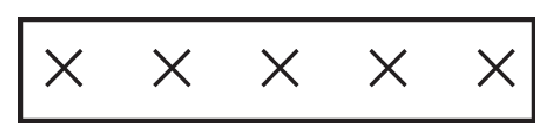
\includegraphics[width=3.5cm]{5X} \\
 USS Gerald R.Ford & 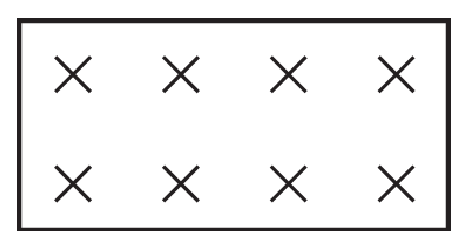
\includegraphics[width=3.5cm]{8X} \\
 \end{tabularx}
 \vspace{0.3cm}
 \item Alternativement chaque équipe répond par raté, touché ou coulé à ses attaquants. L'équipe gagne une fois que tous les bateaux des adversaires sont coulés.
 \end{enumerate}
 
\end{TP}

